\subsection{Architecture Overview}

The MicroNet framework is a collection of components. Each component is
confined in itself which allows simple replacement of components. The components
are organized in three layers: The framework layer, the service catalogue layer,
and the tools layer. \autoref{fig:architecture_layers} shows the layers and all
the components they contain.

\begin{figure}
  \centering
  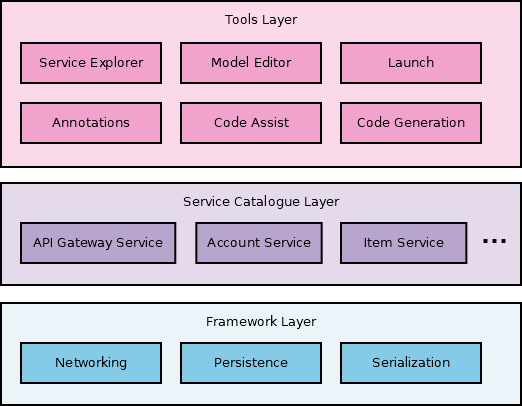
\includegraphics[width=0.7\textwidth]{images/architecture/ArchitectureLayers}
  \caption{The layered architecture of MicroNet with the associated components.}
  \label{fig:architecture_layers}
\end{figure}


The layers and the components they contain are explained below using Component
Responsibility Cards (CRC).

\subsubsection{Framework Layer}

The framework layer provides a uniform interface to the core functionality of
MicroNet.\\

\noindent
\begin{tabular}{|l|l|}
    \cline{1-2}
    \multicolumn{2}{|c|}{} \\[-0.3cm]
    \multicolumn{2}{|c|}{Networking Component} \\ 
    \multicolumn{2}{|c|}{} \\[-0.3cm]
    \cline{1-2}
    Responsibility & Collaboration \\
    \cline{1-2}
    & \\[-0.2cm]
    \begin{minipage}{0.47\textwidth}
        \begin{itemize}
          \item Reliable Messaging System
          \item Connection Authentication
          \item Messaging \gls{api}
        \end{itemize} 
    \end{minipage}
	&
    \begin{minipage}{0.47\textwidth}
        \begin{itemize}
          \item Message Broker (ActiveMQ)
          \item Serialization Component
        \end{itemize} 
    \end{minipage}
	\\ & \\
    \hline
\end{tabular}

\vspace{0.5cm} \noindent 
\begin{tabular}{|l|l|}
    \cline{1-2}
    \multicolumn{2}{|c|}{} \\[-0.3cm]
    \multicolumn{2}{|c|}{Persistence Component} \\ 
    \multicolumn{2}{|c|}{} \\[-0.3cm]
    \cline{1-2}
    Responsibility & Collaboration \\
    \cline{1-2}
    & \\[-0.2cm]
    \begin{minipage}{0.47\textwidth}
        \begin{itemize}
          \item Uniform Database Access
          \item Offer Relational Database 
          \item Offer NoSQL Database
          \item Java \gls{api}
        \end{itemize} 
    \end{minipage}
	&
    \begin{minipage}{0.47\textwidth}
        \begin{itemize}
          \item Relational DBMS (PostgreSQL)
          \item JDBC
          \item NoSQL Database (Couchbase)
        \end{itemize} 
    \end{minipage}
	\\ & \\
    \hline
\end{tabular}

\vspace{0.5cm} \noindent 
\begin{tabular}{|l|l|}
    \cline{1-2}
    \multicolumn{2}{|c|}{} \\[-0.3cm]
    \multicolumn{2}{|c|}{Serialization Component} \\ 
    \multicolumn{2}{|c|}{} \\[-0.3cm]
    \cline{1-2}
    Responsibility & Collaboration \\
    \cline{1-2}
    & \\[-0.2cm]
    \begin{minipage}{0.47\textwidth}
        \begin{itemize}
          \item Uniform Serialization \gls{api}
          \item Make serialization technology interchangeable
          \item \gls{json} serialization
          \item Binary serialization
        \end{itemize} 
    \end{minipage}
	&
    \begin{minipage}{0.47\textwidth}
        \begin{itemize}
          \item Serialization Library (Gson)
        \end{itemize} 
    \end{minipage}
	\\ & \\
    \hline
\end{tabular}

\subsubsection{Service Catalogue Layer}

The service catalogue was a mainly developed in the second semester thesis
\todo{Chapter 5 Prototype Implementation}. This section will exemplary give
three examples of catalogue services.\\

\noindent
\begin{tabular}{|l|l|}
    \cline{1-2}
    \multicolumn{2}{|c|}{} \\[-0.3cm]
    \multicolumn{2}{|c|}{API Gateway Service} \\ 
    \multicolumn{2}{|c|}{} \\[-0.3cm]
    \cline{1-2}
    Responsibility & Collaboration \\
    \cline{1-2}
    & \\[-0.2cm]
    \begin{minipage}{0.47\textwidth}
        \begin{itemize}
          \item Receive and filter requests from clients
          \item Forward requests to \mss{}
          \item Forward Events to clients
          \item Broadcast events to groups of clients
        \end{itemize} 
    \end{minipage}
	&
    \begin{minipage}{0.47\textwidth}
        \begin{itemize}
          \item Account Service (connection authentication)
        \end{itemize} 
    \end{minipage}
	\\ & \\
    \hline
\end{tabular}

\vspace{0.5cm} \noindent 
\begin{tabular}{|l|l|}
    \cline{1-2}
    \multicolumn{2}{|c|}{} \\[-0.3cm]
    \multicolumn{2}{|c|}{Account Service} \\ 
    \multicolumn{2}{|c|}{} \\[-0.3cm]
    \cline{1-2}
    Responsibility & Collaboration \\
    \cline{1-2}
    & \\[-0.2cm]
    \begin{minipage}{0.47\textwidth}
        \begin{itemize}
          \item User Registration
          \item User Authentication
        \end{itemize} 
    \end{minipage}
	&
    \begin{minipage}{0.47\textwidth}
        \begin{itemize}
          \item Account Database (PostgreSQL)
        \end{itemize} 
    \end{minipage}
	\\ & \\
    \hline
\end{tabular}

\vspace{0.5cm} \noindent 
\begin{tabular}{|l|l|}
    \cline{1-2}
    \multicolumn{2}{|c|}{} \\[-0.3cm]
    \multicolumn{2}{|c|}{Item Service} \\ 
    \multicolumn{2}{|c|}{} \\[-0.3cm]
    \cline{1-2}
    Responsibility & Collaboration \\
    \cline{1-2}
    & \\[-0.2cm]
    \begin{minipage}{0.47\textwidth}
        \begin{itemize}
          \item Player Inventory (Carried Items)
          \item Bank (Item Storage)
        \end{itemize} 
    \end{minipage}
	&
    \begin{minipage}{0.47\textwidth}
        \begin{itemize}
          \item Item Database (PostgreSQL)
        \end{itemize} 
    \end{minipage}
	\\ & \\
    \hline
\end{tabular}

\subsubsection{Tools Layer}

The development of the tool layer was a major part of the lab research. The
tools layer's main purpose is to provide aid with the tenet decentralized
continuous delivery. But the tools layer has also the responsibility to adapt
\ms{} application development to be suitable for \og{} development.\\

\noindent
\begin{tabular}{|l|l|}
    \cline{1-2}
    \multicolumn{2}{|c|}{} \\[-0.3cm]
    \multicolumn{2}{|c|}{Annotation Processing} \\ 
    \multicolumn{2}{|c|}{} \\[-0.3cm]
    \cline{1-2}
    Responsibility & Collaboration \\
    \cline{1-2}
    & \\[-0.2cm]
    \begin{minipage}{0.47\textwidth}
        \begin{itemize}
          \item Framework functionality\footnotemark 
          \item Boilerplate code reduction
          \item Defining the shared messaging \gls{api}
        \end{itemize} 
    \end{minipage}
	&
    \begin{minipage}{0.47\textwidth}
        \begin{itemize}
          \item Shared Model (to export the \gls{api})
        \end{itemize} 
    \end{minipage}
	\\ & \\
    \hline
\end{tabular}

\footnotetext{The user code is
          called by the framework (application skeleton) opposed to the user
          code calling a library (well-defined operations).}
          
\vspace{0.5cm} \noindent      
\begin{tabular}{|l|l|}
    \cline{1-2}
    \multicolumn{2}{|c|}{} \\[-0.3cm]
    \multicolumn{2}{|c|}{Code Assist} \\ 
    \multicolumn{2}{|c|}{} \\[-0.3cm]
    \cline{1-2}
    Responsibility & Collaboration \\
    \cline{1-2}
    & \\[-0.2cm]
    \begin{minipage}{0.47\textwidth}
        \begin{itemize}
          \item Present the Shared \gls{api} to the developer
          \item Auto-completion of URIs
          \item Recognize \gls{api} usage errors at compile-time
        \end{itemize} 
    \end{minipage}
	&
    \begin{minipage}{0.47\textwidth}
        \begin{itemize}
          \item Shared Model (to import the \gls{api})
        \end{itemize} 
    \end{minipage}
	\\ & \\
    \hline
\end{tabular}

\vspace{0.5cm} \noindent         
\begin{tabular}{|l|l|}
    \cline{1-2}
    \multicolumn{2}{|c|}{} \\[-0.3cm]
    \multicolumn{2}{|c|}{Code Generation} \\ 
    \multicolumn{2}{|c|}{} \\[-0.3cm]
    \cline{1-2}
    Responsibility & Collaboration \\
    \cline{1-2}
    & \\[-0.2cm]
    \begin{minipage}{0.47\textwidth}
        \begin{itemize}
          \item Generate the MicroNet Framework integration classes
          \item Generate POJOs from the Shared Model
        \end{itemize} 
    \end{minipage}
	&
    \begin{minipage}{0.47\textwidth}
        \begin{itemize}
          \item Shared Model (to import the \gls{api} and Template Types)
          \item Java compiler (annotation processing)
        \end{itemize} 
    \end{minipage}
	\\ & \\
    \hline
\end{tabular}

\vspace{0.5cm} \noindent         
\begin{tabular}{|l|l|}
    \cline{1-2}
    \multicolumn{2}{|c|}{} \\[-0.3cm]
    \multicolumn{2}{|c|}{Service Explorer} \\ 
    \multicolumn{2}{|c|}{} \\[-0.3cm]
    \cline{1-2}
    Responsibility & Collaboration \\
    \cline{1-2}
    & \\[-0.2cm]
    \begin{minipage}{0.47\textwidth}
        \begin{itemize}
          \item Management visual interface for the application (UI)
          \item Compose the application out of catalogue and developed game
          services
        \end{itemize} 
    \end{minipage}
	&
    \begin{minipage}{0.47\textwidth}
        \begin{itemize}
          \item Service Catalogue
          \item Launch Utility (to provide the UI)
        \end{itemize} 
    \end{minipage}
	\\ & \\
    \hline
\end{tabular}

\vspace{0.5cm} \noindent      
\begin{tabular}{|l|l|}
    \cline{1-2}
    \multicolumn{2}{|c|}{} \\[-0.3cm]
    \multicolumn{2}{|c|}{Model Editor} \\ 
    \multicolumn{2}{|c|}{} \\[-0.3cm]
    \cline{1-2}
    Responsibility & Collaboration \\
    \cline{1-2}
    & \\[-0.2cm]
    \begin{minipage}{0.47\textwidth}
        \begin{itemize}
          \item Define and edit the shared model as template types
          \item Instantiate templates as prefabs
          \item Synchronize the Shared Model between developers
        \end{itemize} 
    \end{minipage}
	&
    \begin{minipage}{0.47\textwidth}
        \begin{itemize}
          \item Shared Model (CRUD)
          \item Database Component (for sharing)
        \end{itemize} 
    \end{minipage}
	\\ & \\
    \hline
\end{tabular}

\vspace{0.5cm} \noindent        
\begin{tabular}{|l|l|}
    \cline{1-2}
    \multicolumn{2}{|c|}{} \\[-0.3cm]
    \multicolumn{2}{|c|}{Launch Utility} \\ 
    \multicolumn{2}{|c|}{} \\[-0.3cm]
    \cline{1-2}
    Responsibility & Collaboration \\
    \cline{1-2}
    & \\[-0.2cm]
    \begin{minipage}{0.47\textwidth}
        \begin{itemize}
          	\item Build the composed application
			\item Simplify application deployment
          	\item Provide launch configurations for local deployments 
        \end{itemize} 
    \end{minipage}
	&
    \begin{minipage}{0.47\textwidth}
        \begin{itemize}
          \item Maven (build)
          \item Docker (build \& run)
          \item Docker-compose (compose the application)
          \item optionally uses CDT Launch Groups and Eclipse Docker Tools
        \end{itemize} 
    \end{minipage}
	\\ & \\
    \hline
\end{tabular}
